\documentclass{beamer}
\mode<presentation>{
\usetheme{Amsterdam}
\setbeamertemplate{navigation symbols}{}}
\usepackage[utf8]{inputenc}
\usepackage{graphicx}
\usepackage{booktabs}
\usepackage{listings}
\usepackage{color}

\definecolor{mygreen}{rgb}{0,0.6,0}
\definecolor{mygray}{rgb}{0.5,0.5,0.5}
\definecolor{mymauve}{rgb}{0.58,0,0.82}

\lstset{ %
  backgroundcolor=\color{white},   % choose the background color
  basicstyle=\footnotesize,        % size of fonts used for the code
  breaklines=true,                 % automatic line breaking only at whitespace
  captionpos=b,                    % sets the caption-position to bottom
  commentstyle=\color{mygreen},    % comment style
  escapeinside={\%*}{*)},          % if you want to add LaTeX within your code
  keywordstyle=\color{blue},       % keyword style
  stringstyle=\color{mymauve},     % string literal style
}


%----------------------------------------------------------------------------------------
%	TITULOS
%----------------------------------------------------------------------------------------
\title[Seminario de tecnologia]{Unidad III\\ Microcontroladores}
\author{David A. Trejo Pizzo}
\institute[Instituto Multimedial Da Vinci]
{Departamento de sistemas\\
\medskip
\textit{dtrejopizzo@gmail.com}}
\date{Marzo, 2015}
\begin{document}
\begin{frame}
\titlepage
\end{frame}


%----------------------------------------------------------------------------------------
%	INDICE
%----------------------------------------------------------------------------------------
\begin{frame}
\frametitle{Estructura}
\tableofcontents
\end{frame}


%----------------------------------------------------------------------------------------
%	SLIDES
%----------------------------------------------------------------------------------------

\section{Introducción}

\begin{frame}
\frametitle{Que es un microcontrolador?}
\begin{itemize}
\item Un microcontrolador es un circuito integrado que incorpora en su interior un procesador, memorias y una serie de periféricos que lo hacen apto para desempeñar distintas funciones.
\item Su funcionamiento depende del programa que tenga cargado en su memoria.
\end{itemize}
%\begin{figure}[!h]
%\centering
%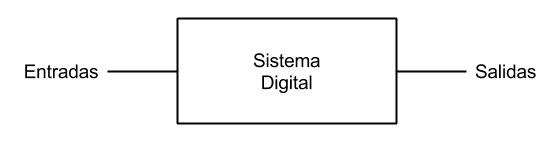
\includegraphics[width=2in]{sistemad}
%\end{figure}
\end{frame}
%------------------------------------------------

\begin{frame}
\frametitle{Componentes}
\begin{itemize}
\item Unidad de control
\item Conjunto de registros
\item Unidad aritmético y lógica
\item Buses de conexión
\item Unidad  de cálculo de coma flotante
\end{itemize}
\end{frame}
%------------------------------------------------

\begin{frame}
\frametitle{Que es un microcontrolador?}
\begin{figure}[!h]
\centering
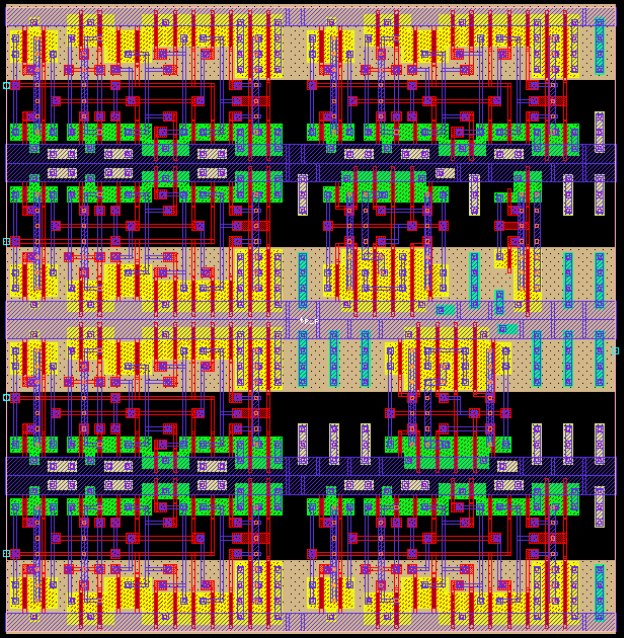
\includegraphics[width=2.5in]{ocp-22}
\end{figure}
\end{frame}
%------------------------------------------------

\section{AVR}
\begin{frame}
\frametitle{Core}
\begin{figure}[!h]
\centering
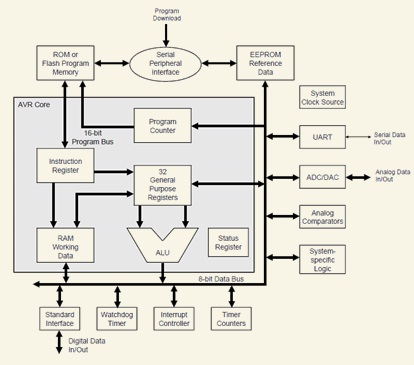
\includegraphics[width=2in]{avrcore}
\end{figure}
\end{frame}
%------------------------------------------------

\begin{frame}
\frametitle{Implementacion fisica}
\begin{figure}[!h]
\centering
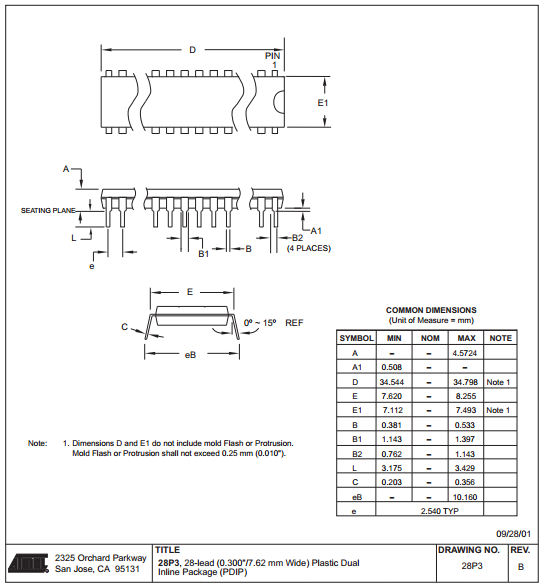
\includegraphics[width=2in]{dibujo}
\end{figure}
\end{frame}
%------------------------------------------------

\begin{frame}
\frametitle{AVR}
El AVR fue diseñado desde un comienzo para la ejecución eficiente en lenguaje C.\\

La familia de microcontroladores es bastante numerosa, con más de 70 dispositivos y variantes que poseen el mismo núcleo; solo varían la cantidad de memoria y los periféricos.
\begin{figure}[!h]
\centering
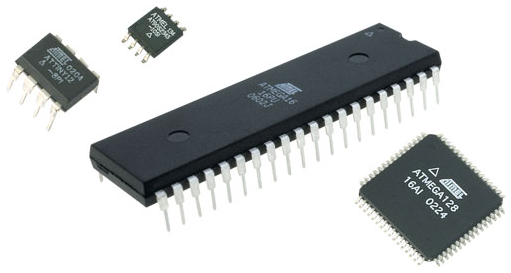
\includegraphics[width=2in]{micros}
\end{figure}
\end{frame}
%------------------------------------------------

\begin{frame}
\frametitle{Periféricos}
\begin{itemize}
\item Puertos de Entradas / Salidas
\item Timers
\item Generador de interrupciones
\item Interfaces de comunicación
\item Conversor Analógico / Digital
\item Conversor Digital / Analógico
\end{itemize}
\end{frame}
%------------------------------------------------

\begin{frame}
\frametitle{Memoria y periféricos}
El tipo y cantidad de periféricos, va a depender de cada fabricante. Lo mismo el tamaño y tipo de las memorias.\\

Se debe elegir al microcontrolador de acuerdo a las necesidades del proyecto a implementar.\\

Los fabricantes ofrecen cuadros comparativos entre sus distintas familias,  los cuales permiten ver de forma detallada las distintas características de cada producto.
\end{frame}
%------------------------------------------------

\begin{frame}
\frametitle{Arquitectura RISC}
\begin{quotation}
Reduced COMPLEXITY Instruction Set Computer.
\end{quotation}
No significa un número de instrucciones reducido como a menudo se piensa. Significa que se reduce la complejidad de los circuitos encargados de la decodificación de las instrucciones , haciéndolos más simples y eficientes. 
\end{frame}
%------------------------------------------------

\begin{frame}
\frametitle{ARV RISC}
\begin{itemize}
\item Utiliza instrucciones de tamaño fijo. Solo 4 instrucciones de 32 bits y el resto son de 16 bits
\item Posee 32 registros de uso general
\item Solo utiliza instrucciones de Load/Store para acceder a la memoria RAM.
\item La mayoría de las instrucciones se ejecutan en 1 ciclo de clock.
\item Esta diseñada especialmente para la programación en C.
\item Posee muy buenas características de bajo consumo
\end{itemize}
\end{frame}
%------------------------------------------------

\begin{frame}
\frametitle{Arquitectura AVR}
\begin{figure}[!h]
\centering
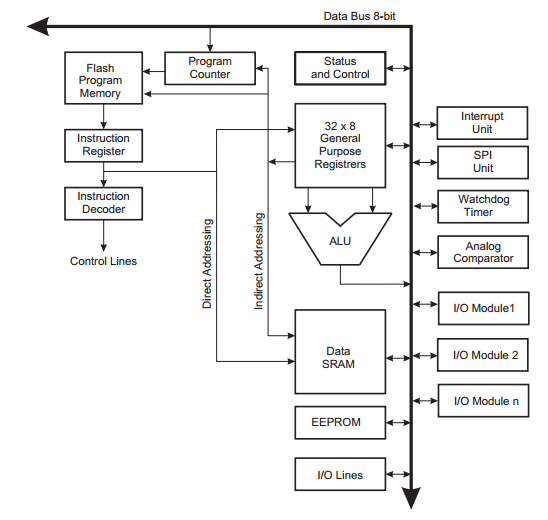
\includegraphics[width=2in]{avrarch}
\end{figure}
\end{frame}
%------------------------------------------------

\begin{frame}
\frametitle{Ciclos}
En un ciclo de reloj se pueden leer 2 registros que funcionen como operandos para la ALU, realizar la operación y que le resultado quede disponible para escribirse en uno de esos registros.
\begin{figure}[!h]
\centering
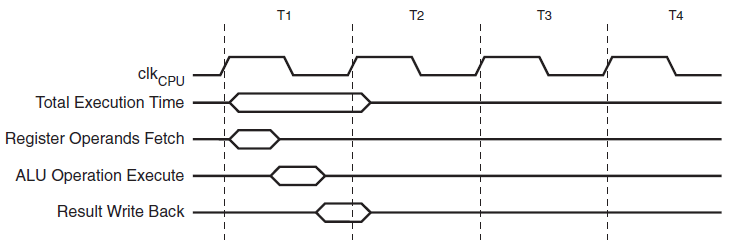
\includegraphics[width=3in]{ciclos}
\end{figure}
\end{frame}
%------------------------------------------------

\begin{frame}
\frametitle{Bus de comunicaciones}
\begin{itemize}
\item La arquitectura de un microcontrolador no solo está definida por su set de instrucciones, sino también por la arquitectura del bus de comunicaciones.
\item Arquitectura de Von Newmann: los buses de acceso a la memoria de programa y a la memoria de datos son los mismos, resultando así un único mapa de memoria.
\item Arquitectura Harvard: se utilizan buses separados para la memoria de programa y la de datos.
\end{itemize}
\begin{quotation}
Los microcontroladores AVR poseen una Arquitectura Harvard.
\end{quotation}
\end{frame}
%------------------------------------------------

\section{Programacion}

\begin{frame}
\frametitle{El lenguaje C}

\end{frame}
%------------------------------------------------

\begin{frame}
\frametitle{El lenguaje C modificado}

\end{frame}
%------------------------------------------------

\subsection{Operadores y tipos de datos}

\begin{frame}
\frametitle{Operadores}
\begin{columns}[c]
\column{.5\textwidth}
Aritmeticos
\begin{itemize}
\item = (asignar)
\item + (suma)
\item - (resta)
\item * (multriplicacion)
\item / (division)
\item \% (modulo)
\end{itemize}
\column{.5\textwidth}
Comparacion
\begin{itemize}
\item == (igual a)
\item != (distinto a)
\item $<$ (menor que)
\item $>$ (mayor que)
\item $<=$ (menor o igual que)
\item $>=$ (mayor o igual que)
\end{itemize}
Boleanos
\begin{itemize}
\item $\&\&$ (y)
\item $||$ (o)
\item ! (no)
\end{itemize}
\end{columns}
\end{frame}
%------------------------------------------------

\begin{frame}
\frametitle{Otros operadores}
\begin{columns}[c]
\column{.5\textwidth}
Compuestos
\begin{itemize}
\item ++ (incremento)
\item -- (decrementar)
\end{itemize}
Punteros
\begin{itemize}
\item * desreferencia
\item $\&$ referencia
\end{itemize}
\column{.5\textwidth}
Bit a bit
\begin{itemize}
\item $\&$ (y)
\item $|$ (o)
\item $\wedge$ (xor)
\item $\sim$ (no)
\item $<<$ (bit shift a la izquierda)
\item $>>$ (bit shift a la derecha)
\end{itemize}
\end{columns}
\end{frame}
%------------------------------------------------

\begin{frame}
\frametitle{Tipos de datos}
\begin{columns}[c]
\column{.5\textwidth}
\begin{itemize}
\item void
\item booleano
\item char
\item unsigned char
\item byte
\item int
\item unsigned int
\end{itemize}
\column{.5\textwidth}
\begin{itemize}
\item word
\item long
\item unsigned long
\item short
\item float
\item double
\item string (char[])
\item String (objeto)
\item array
\end{itemize}
\end{columns}
\end{frame}
%------------------------------------------------

\subsection{Sentencias de control}

\begin{frame}[fragile]
\frametitle{Sentencia IF}
\begin{itemize}
\item Si $X \longrightarrow Y$
\begin{lstlisting}[language=java]
if (X) {
   // Y}
\end{lstlisting}

\item Si $X \longrightarrow Y \vee Z$
\begin{lstlisting}[language=java]
if (X) {
   // Y}
else {
   // Z}
\end{lstlisting}

\item Si $W \longrightarrow X \vee Y \longrightarrow Z$
\begin{lstlisting}[language=java]
if (W) {
   // X}
else if (Y) {
   // Z}
\end{lstlisting}
\end{itemize}
\end{frame}
%------------------------------------------------

\begin{frame}[fragile]
\frametitle{Switch}
La estructura \textbf{Switch} funciona como un menu. Cuando se encuentra una sentencia \textbf{case} cuyo valor coincide con el de la variable, se ejecuta el código en esa declaración de caso.
\vspace{0.1in}
\begin{columns}[c]
\column{.5\textwidth}
Sintaxis:\\
\begin{lstlisting}[language=java]
switch (var) {
  case label:
    // statements
    break;
  case label:
    // statements
    break;
  default: 
    // statements
}
\end{lstlisting}
\column{.5\textwidth}
Ejemplo:
\begin{lstlisting}[language=java]
switch (var) {
    case 1:
      //do
      break;
    case 2:
      //do
      break;
    default:
  }
\end{lstlisting}
\end{columns}
\end{frame}
%------------------------------------------------

\begin{frame}[fragile]
\frametitle{Sentencia FOR}
\begin{figure}[!h]
\centering
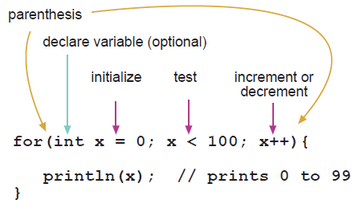
\includegraphics[width=2in]{for}
\end{figure}
\begin{lstlisting}[language=java]

void loop()
{
   for (int i=0; i <= 255; i++)
   {
      analogWrite(10, i);
      delay(10);
   } 
}
\end{lstlisting}
\end{frame}
%------------------------------------------------

\begin{frame}[fragile]
\frametitle{While}
El ciclo \textbf{While} se repetirá de forma continua hasta que la expresión dentro del paréntesis sea falsa.
\vspace{0.1in}
\begin{columns}[c]
\column{.5\textwidth}
Sintaxis:\\
\begin{lstlisting}[language=java]
while(expresion){
  // tarea(s)
}
\end{lstlisting}
\column{.5\textwidth}
Ejemplo:
\begin{lstlisting}[language=java]
var = 0;
while(var < 200){
  var++;
}
\end{lstlisting}
\end{columns}
\end{frame}
%------------------------------------------------

\begin{frame}[fragile]
\frametitle{Do while}
El ciclo \textbf{Do while} es similar al ciclo While, con la excepción de que la condición se comprueba al final del bucle, por lo que el bucle se ejecutará al menos una vez.
\vspace{0.1in}
\begin{columns}[c]
\column{.5\textwidth}
Sintaxis:\\
\begin{lstlisting}[language=java]
do
{
    // statement block
} while (test condition);
\end{lstlisting}
\column{.5\textwidth}
Ejemplo:
\begin{lstlisting}[language=java]
do
{
  delay(50);          
  x = readSensors();
} while (x < 100);
\end{lstlisting}
\end{columns}
\end{frame}
%------------------------------------------------

\subsection{Declaraciones}

\begin{frame}[fragile]
\frametitle{Break}
\begin{columns}[c]
\column{.5\textwidth}
La declaración \textbf{Break} se usa para salir de un ciclo \textbf{do}, \textbf{for} o \textbf{while}, saltando la condicion normal del ciclo.
\column{.5\textwidth}
Ejemplo:
\begin{lstlisting}[language=java]
for (x = 0; x < 255; x ++)
{
    digitalWrite(PWMpin, x);
    sens = analogRead(0);  
    if (sens > threshold){
       x = 0;
       break;
    }  
    delay(50);
}
\end{lstlisting}
\end{columns}
\end{frame}
%------------------------------------------------

\begin{frame}[fragile]
\frametitle{Continue}
\begin{columns}[c]
\column{.5\textwidth}
La declaración \textbf{Continue} se usa para salir de un ciclo \textbf{do}, \textbf{for} o \textbf{while}, saltando el resto del ciclo.
\column{.5\textwidth}
Ejemplo:
\begin{lstlisting}[language=java]
for (x = 0; x < 255; x ++)
{
    if (x > 40 && x < 120){
        continue;
    }
    digitalWrite(PWMpin, x);
    delay(50);
}
\end{lstlisting}
\end{columns}
\end{frame}
%------------------------------------------------

\begin{frame}[fragile]
\frametitle{Return}
\begin{columns}[c]
\column{.5\textwidth}
La declaración \textbf{Return} se usa para terminar una función y retornar un valor a otra funcon o al programa principal.
\column{.5\textwidth}
Ejemplo:
\begin{lstlisting}[language=java]
int checkSensor(){  
	v = analogRead(0);     
    if (v > 400) {
        return 1;
    else{
        return 0;
    }
}
\end{lstlisting}
\end{columns}
\end{frame}
%------------------------------------------------

\begin{frame}[fragile]
\frametitle{Goto}
La declaración \textbf{Goto} transfiere el flujo del programa a otro punto.\\

\vspace{0.2in}
Ejemplo:
\begin{lstlisting}[language=java]
for(byte r = 0; r < 255; r++){
    for(byte g = 255; g > -1; g--){
        for(byte b = 0; b < 255; b++){
            if (analogRead(0) > 250){ goto bailout;}
            // otras declaraciones ... 
        }
    }
}
bailout:
\end{lstlisting}
\end{frame}
%------------------------------------------------



\begin{frame}[fragile]
\frametitle{Sentencia FOR}
\begin{lstlisting}[language=java]
int PWMpin = 10; // LED in series with 470 ohm resistor on pin 10

void setup()
{
  // no setup needed
}

void loop()
{
   for (int i=0; i <= 255; i++){
      analogWrite(PWMpin, i);
      delay(10);
   } 
}
\end{lstlisting}
\end{frame}
%------------------------------------------------

\begin{frame}[fragile]
\frametitle{}
\begin{lstlisting}[language=java]

\end{lstlisting}
\end{frame}
%------------------------------------------------

\begin{frame}[fragile]
\frametitle{}
\begin{lstlisting}[language=java]

\end{lstlisting}
\end{frame}
%------------------------------------------------

\begin{frame}[fragile]
\frametitle{}
\begin{lstlisting}[language=java]

\end{lstlisting}
\end{frame}
%------------------------------------------------

\section{Conversor A-D}

\begin{frame}
\frametitle{El conversor analogico-digital}
\begin{itemize}
\item Un conversor Analógico a Digital (o ADC)  transforma una señal analógica a un número binario.
\item La cantidad de dígitos binarios definen la resolución del ADC.
\item Este número digital es solo una aproximación de la señal analógica, dado que solo puede ser representada en pasos discretos.
\item La exactitud de la conversión dependerá también de la resolución del ADC.
\end{itemize}
\end{frame}
%------------------------------------------------

\begin{frame}
\frametitle{Tipos}
\begin{itemize}
\item Simple o doble rampa.
\item Tipo FLASH
\item De aproximaciones sucesivas.
\item VCO ADC
\item Sigma Delta.
\end{itemize}
\end{frame}
%------------------------------------------------

\begin{frame}
\frametitle{El ADC del ATmega328}
\begin{itemize}
\item 10 bits de resolución
\item 8 canales en modo común multiplexados
\item Hasta 7 canales en modo diferencial.
\item Hasta 15KSPS
\item Referencia seleccionable (Externa o 2.56V internos) 
\item Interrupción al completar la conversión.
\end{itemize}
\end{frame}
%------------------------------------------------

\begin{frame}
\frametitle{Esquema interno}
\begin{figure}[!h]
\centering
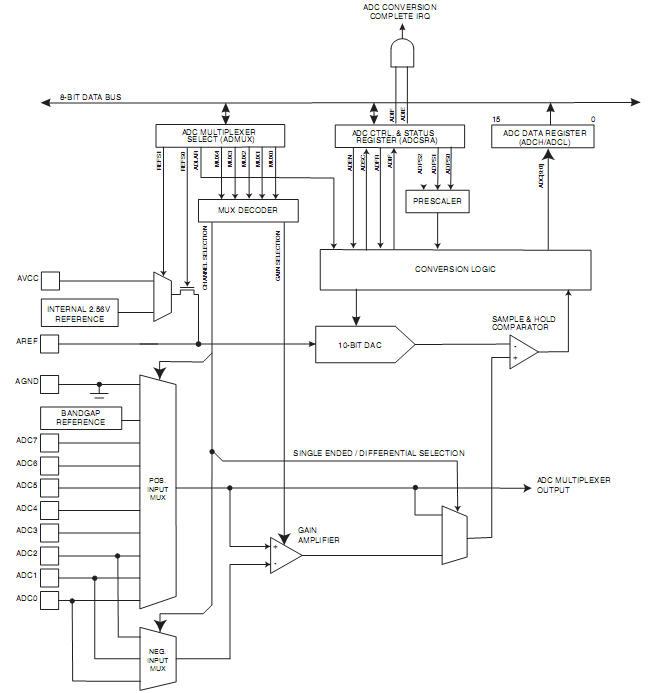
\includegraphics[width=2in]{adc}
\end{figure}
\end{frame}
%------------------------------------------------

\subsection{Modos de conversión}
\begin{frame}
\frametitle{Conversión en Modo comun}
El resultado de la conversión en modo común responde a la siguiente fórmula:

$$ADC  =\frac{V_{IN}*1024}{V_{REF}}$$

Por ejemplo, si $V_{REF}=2.56V$ y la entrada $V_{IN}=1V$, el resultado de la conversión es 400.
\end{frame}
%------------------------------------------------

\begin{frame}
\frametitle{Conversión en modo diferencial}
El resultado de la conversión en modo diferencial responde a la siguiente fórmula:

$$ADC  =\frac{(V_{POS}-V_{NEG})*GAIN*512}{V_{REF}}$$

Es presentado en complemento a 2, desde -512 (ADCH=02h y ADCL=00h) hasta +511 (ADCH=01h y ADCL=FFh).
La polaridad del resultado puede obtenerse leyendo el 2do LSB del registro ADCH.
\end{frame}
%------------------------------------------------

\begin{frame}
\frametitle{}

\end{frame}
%------------------------------------------------

\begin{frame}
\frametitle{}

\end{frame}
%------------------------------------------------

\section{ATmega328}

\begin{frame}
\frametitle{Pinout}
\begin{figure}[!h]
\centering
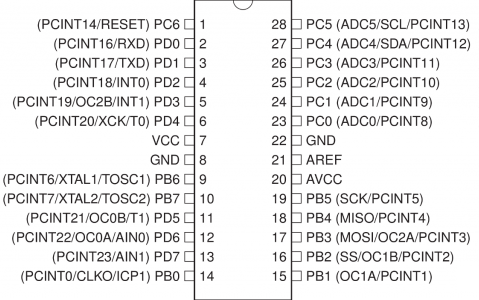
\includegraphics[width=2in]{pinout}
\end{figure}
\end{frame}
%------------------------------------------------

\begin{frame}
\frametitle{Esquema de pines}
\begin{figure}[!h]
\centering
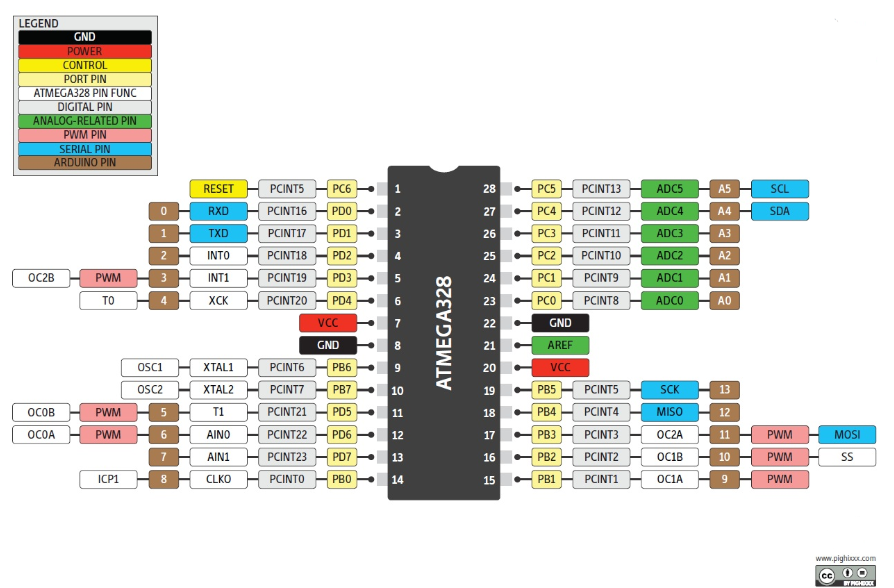
\includegraphics[width=3.5in]{atmega328}
\end{figure}
\end{frame}
%------------------------------------------------



\subsection{Puertos analogicos}

\begin{frame}[fragile]
\frametitle{Lectura analogica}
\begin{lstlisting}[language=java]

void setup() {
  Serial.begin(9600);
}

void loop() {
  int sensorValue = analogRead(A0);
  Serial.println(sensorValue);
}
\end{lstlisting}
\end{frame}
%------------------------------------------------

\begin{frame}[fragile]
\frametitle{}
\begin{lstlisting}[language=java]

\end{lstlisting}
\end{frame}
%------------------------------------------------

\begin{frame}
\frametitle{}

\end{frame}
%------------------------------------------------
\end{document}